\documentclass[
12pt, % Main document font size
a4paper, % Paper type, use 'letterpaper' for US Letter paper
oneside, % One page layout (no page indentation)
%twoside, % Two page layout (page indentation for binding and different headers)
%hidelinks, % Hide links like hyperref
%headinclude,footinclude, % Extra spacing for the header and footer
%BCOR5mm, % Binding correction
]{article}



%\setlength{\parindent}{0pt} %Modifica la dimensione dell'indentazione dei paragrafi



\hyphenation{Fortran hy-phen-ation se-mi-auto-no-} 


%%%%% Packages
\usepackage [italian]{babel}
%\usepackage [english]{babel}
\usepackage [autostyle, english = american]{csquotes}
\MakeOuterQuote{"}

\usepackage[section]{placeins} %Also one can consider the placeins package and the \FloatBarrier command that prevents figures from floating any further. If figures are supposed to remain in the section, one can load

\usepackage{graphicx}
\usepackage{subfig}
\usepackage{xcolor} %Colori Aggiuntiv
\usepackage[colorlinks = true,
	linkcolor = teal,
	urlcolor  = blue,
	citecolor = blue,
	anchorcolor = blue]{hyperref} %Hyperref
	
\usepackage{url}

%\usepackage{lipsum} %Crea dummy text

\usepackage{amsmath,amssymb,amscd,amsfonts,amsthm,amsrefs} %Roba matematica
\usepackage{mathtools}

\usepackage{physics}

\usepackage{siunitx} %database unita` di misura, \si{ \kg \per \second},  \SI{20}{ \kg \per \second}

\usepackage{gensymb} %simboli extra, come \degree

\usepackage{tikz}
	\usetikzlibrary{shapes,arrows}
	\tikzstyle{block} = [draw, fill=white, rectangle, 
	minimum height=3em, minimum width=6em]
	\tikzstyle{sum} = [draw, fill=white, circle, node distance=1cm]
	\tikzstyle{input} = [coordinate]
	\tikzstyle{output} = [coordinate]
	\tikzstyle{pinstyle} = [pin edge={to-,thin,black}]
	\usepackage{tikzscale}

\usepackage{pgfplots}
	\pgfplotsset{width=7cm,compat=1.14}
	%\pgfplotsset{compat=newest} % Allows to place the legend below plot
	\pgfplotsset{every minor tick/.append style={thin}}  % applies only to minor ticks,
	\usepgfplotslibrary{units} % Allows to enter the units nicely
	%\usepgfplotslibrary{external} 
	%\tikzexternalize
	%\tikzset{external/force remake}
	\pgfkeys{/pgf/number format/.cd,1000 sep={\,}}

\sisetup{
	round-mode          = places,
	round-precision     = 2,
}



\usepackage{afterpage}

\newcommand\blankpage{%
	\null
	\thispagestyle{empty}%
	%\addtocounter{page}{-1}%
	\newpage}
%per creare pagine vuote

\usepackage{vmargin}
\setmarginsrb  {25mm}  % left margin
	{ 5mm}  % top margin
	{25mm}  % right margin
	{15mm}  % bottom margin
	{10mm}  % head height
	{15mm}  % head sep
	{10mm}  % foot height
	{15mm}  % foot sep

\setpapersize{A4}


%%%%%%%%%%%%%%%%%%%%%%%%%%%%%%%%%%%%%%%%%%%%%%%%%%%%%%%%%%
%%%%% Comandi homebrewed

\newcommand{\at}[2][]{#1|_{#2}} %Comando per le derivate calcolate nel punto. Esempio: \dv{\text{Im}T(j \omega)}{t} \at[\Big]{\omega = \omega_1}

%% Comando per valori assoluti che scalano
%\DeclarePairedDelimiter\abs{\lvert}{\rvert}%
%\DeclarePairedDelimiter\norm{\lVert}{\rVert}%
% Swap the definition of \abs* and \norm*, so that \abs
% and \norm resizes the size of the brackets, and the 
% starred version does not.
\makeatletter
\let\oldabs\abs
\def\abs{\@ifstar{\oldabs}{\oldabs*}}
%
\let\oldnorm\norm
\def\norm{\@ifstar{\oldnorm}{\oldnorm*}}
\makeatother

\DeclarePairedDelimiter\ceil{\lceil}{\rceil}
\DeclarePairedDelimiter\floor{\lfloor}{\rfloor}

%% Prova theorem
\newtheorem{theorem}{Theorem}[section]
\newtheorem{lemma}[theorem]{Lemma}
\newtheorem{proposition}[theorem]{Proposition}
\newtheorem{corollary}[theorem]{Corollary}

\newenvironment{Proof}[1][Proof]{\begin{trivlist}
		\item[\hskip \labelsep {\bfseries #1}]}{\end{trivlist}}
\newenvironment{definition}[1][Definition]{\begin{trivlist}
		\item[\hskip \labelsep {\bfseries #1}]}{\end{trivlist}}
\newenvironment{example}[1][Example]{\begin{trivlist}
		\item[\hskip \labelsep {\bfseries #1}]}{\end{trivlist}}
\newenvironment{remark}[1][Remark]{\begin{trivlist}
		\item[\hskip \labelsep {\bfseries #1}]}{\end{trivlist}}

%\newcommand{\qed}{\nobreak \ifvmode \relax \else
%	\ifdim\lastskip<1.5em \hskip-\lastskip
%	\hskip1.5em plus0em minus0.5em \fi \nobreak
%	\vrule height0.75em width0.5em depth0.25em\fi}




\graphicspath{{./figs/}}
\pgfplotsset{
	table/search path={./figs},
}

\title{\normalfont{Simulazione e Controllo del Pendolo Inverso di Furuta}}
\author{Francesco Petracci e Simone Silenzi} 


\begin{document}
	
\begin{titlepage}
	\centering
	\vspace*{2 cm}
	\textsc{\Large Universit\`a di Pisa }\\[0.5 cm]							% University Name
	%\textsc{\Large Scuola di Ingegneria}\\[0.5 cm]		
	\textsc{\large Corso di Laurea magistrale \\ 
		\vspace*{3mm} in Ingegneria Robotica e dell'Automazione}\\[1 cm]		% Course Code
	\rule{\linewidth}{0.2 mm} \\
	{ \Large{\textbf{Simulazione e Controllo \\ del Pendolo Inverso di Furuta}}}\\
	
	\rule{\linewidth}{0.2 mm} \\[2.5 cm]
%	\vspace*{1.5 cm}
	
	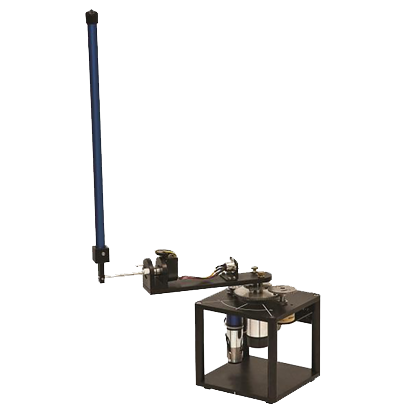
\includegraphics[height=.35\textheight]{quanser_furuta.png}
	
	\vspace*{2 cm}
	\begin{minipage}{0.48\textwidth}
		\begin{flushleft}
			\textit{Autori:}\\
			Francesco Petracci\\
			Simone Silenzi
		\end{flushleft}
	\end{minipage}~
	\begin{minipage}{0.48\textwidth}
		\begin{flushright}
			\textit{Matricola e-mail:}\\		
			491648, \href{mailto:petracci.francesco@gmail.com}{petracci.francesco@gmail.com} \\
			460123, \href{mailto:s.silenzi1@gmail.com}{s.silenzi1@gmail.com}
		\end{flushright}
	\end{minipage}\\[2 cm]
	
%	\textit{Autori, matricola ed email:} \\
%	Francesco Petracci, 491648, \href{mailto:petracci.francesco@gmail.com}{petracci.francesco@gmail.com} \\
%	Simone Silenzi, 460123, \href{mailto:s.silenzi1@gmail.com}{s.silenzi1@gmail.com} \\
	
	
\end{titlepage}
\newpage

\section{Indicazioni Report}
Project reportA  report  must  be  produced  (8-10  pages)  to  explain  the  project  details.  In  particular,  the  title  page  must  contain  the  name  of  the  course  under  which  the  project  has  been  done,  the  project  title,  an  optional  picture related  to  the  project,  the  delivery  date,  and the  author(s)  name(s)  with  contact  information (student ID number and Email). The  report  must  include  a  general  description  of  the  project,  the  physical  model  used,  the  design  choices, the user interface, the shared data structures, the tasks involved, a task-resource diagram, a discussion  on  the  task  parameters  (how they  were  defined),  and  a  set  of  experimental  results  that show  the  behavior  of  the  system  as  a  function  of  specific  variables.  Figures  and  screen  shots  are  welcome. The project code must not be included in the report, but in a separate folder.
 
\section{Introduzione}
Questo progetto consiste nella simulazione dell'interazione real-time tra il pendolo inverso di Furuta, una scheda STM32F4 Discovery e un'interfaccia utente su pc. 

L'applicazione finale \`e stata sviluppata in C sfruttando principalmente le librerie Allegro e Pthread. Per quanto riguarda la simulazione del pendolo e della scheda \`e stato fatto uso del software \textsc{Matlab--Simulink} per sviluppare un modello fisico, il relativo controllo e per quindi creare in modo automatico alcune funzioni.


\section{cose Simone}
\begin{math}\\
T=\dfrac{1}{2} \left(2  L_{arm} l_p m_p \dot{\alpha } \dot{\theta } \cos (\theta ) + \left(J_0 + J_p\sin ^2(\theta )\right) \dot{\alpha }^2+ J_p \dot{\theta }^2\right)\\
U=g l_p m_p (\cos(\theta) - 1)\\
M(q)\ddot{q}+C(q,\dot{q})\dot{q}+N(q,\dot{q})=\tau\\
q=\left( \begin{array}{cc}\alpha & \theta\\\end{array}\right)^{T}\\
M(q)=\left(\begin{array}{cc}\dfrac{\partial^{2} T}{\partial \dot{\alpha }^{2} } & \dfrac{\partial^{2} T}{\partial \dot{\alpha } \partial \dot{\theta } }\\
\dfrac{\partial^{2} T}{\partial \dot{\alpha } \partial \dot{\theta } } & \dfrac{\partial^{2} T}{\partial \dot{\theta }^{2} }\\
\end{array}\right)=\left(\begin{array}{cc}
J_0+J_p \sin ^2(\theta ) & L_{arm} l_p m_p \cos (\theta ) \\
L_{arm} l_p m_p \cos (\theta ) & J_p \\
\end{array}\right)\\
C(q,\dot{q})= \dfrac{1}{2}\left(
\begin{array}{cc}
\dfrac{\partial M_{11}}{\partial \alpha}\dot{\alpha } + \dfrac{\partial M_{11}}{\partial \theta}\dot{\theta } &
\dfrac{\partial M_{11}}{\partial \theta}\dot{\alpha } + (2 \dfrac{\partial M_{12}}{\partial \theta} - \dfrac{\partial M_{22}}{\partial \alpha})\dot{\theta } \\
(2 \dfrac{\partial M_{21}}{\partial \alpha} - \dfrac{\partial M_{11}}{\partial \theta}) \dot{\alpha } + \dfrac{\partial M_{22}}{\partial \alpha} \dot{\theta } &
\dfrac{\partial M_{22}}{\partial \alpha} \dot{\alpha } + \dfrac{\partial M_{22}}{\partial \theta} \dot{\theta }\\
\end{array}\right) = \left(	\begin{array}{cc}\dfrac{1}{2} J_p \dot{\theta } \sin (2 \theta )& \dfrac{1}{2} J_p \dot{\alpha } \sin (2 \theta )-L_{arm} l_p m_p\dot{\theta } \sin (\theta ) \\
-\dfrac{1}{2} J_p \dot{\alpha } \sin (2 \theta ) & 0 \\
\end{array}
\right)\\
N(q,\dot{q})=\left(\begin{array}{c}b_{ma}\dot{\alpha } + \dfrac{\partial U}{\partial \alpha }\\
b_p \dot{\theta } + \dfrac{\partial U}{\partial \theta }\\
\end{array}\right)=\left(\begin{array}{c}
b_{ma} \dot{\alpha }\\
b_p \dot{\theta } -g l_p m_p \sin (\theta )\\
\end{array}\right)\\
\ddot{q}={M(q)}^{-1}(\tau-C(q,\dot{q})\dot{q}-N(q,\dot{q}))\\
\left(\begin{array}{c}\ddot{\alpha}\\
\ddot{\theta}\\
\end{array}\right) ={\left(\begin{array}{cc}
	J_0+J_p \sin ^2(\theta ) & L_{arm} l_p m_p \cos (\theta ) \\
	L_{arm} l_p m_p \cos (\theta ) & J_p \\
	\end{array}\right)}^{-1}\left(\left(\begin{array}{c}\tau_1\\\tau_2\\\end{array}\right)-\left(
\begin{array}{cc}\dfrac{1}{2} J_p \dot{\theta } \sin (2 \theta )&\dfrac{1}{2} J_p \dot{\alpha } \sin (2 \theta )-L_{arm} l_p m_p\dot{\theta } \sin (\theta ) \\
-\dfrac{1}{2} J_p \dot{\alpha } \sin (2 \theta ) & 0 \\
\end{array}
\right)\left( \begin{array}{c}\dot{\alpha}\\
\dot{\theta}\\
\end{array}\right)-\left(\begin{array}{c}
b_{ma} \dot{\alpha }\\
b_p \dot{\theta } -g l_p m_p \sin (\theta )\\
\end{array}\right)\right)
%	=\\=\left(\begin{array}{c}
%		\dfrac{2 \dot{\theta } L_{arm} b_p \cos (\theta ) l_p m_p-2 g L_{arm} \sin
%			(\theta ) \cos (\theta ) l_p^2 m_p^2+\dot{\alpha }^2 L_{arm} \sin (2 \theta )
%			(-\cos (\theta )) J_p l_p m_p+2 \dot{\theta }^2 L_{arm} \sin (\theta ) J_p l_p
%			m_p-2 \tau _2 L_{arm} \cos (\theta ) l_p m_p-2 \dot{\alpha } b_{ma} J_p-2
%			\dot{\alpha } \dot{\theta } \sin (2 \theta ) J_p^2+2 \tau _1 J_p}{2
%			\left(-L_{arm}^2 \cos ^2(\theta ) l_p^2 m_p^2+\sin ^2(\theta ) J_p^2+J_0
%			J_p\right)} \\
%		\dfrac{2 \dot{\alpha } L_{arm} b_{ma} \cos (\theta ) l_p m_p+2 \dot{\alpha }
%			\dot{\theta } L_{arm} \sin (2 \theta ) \cos (\theta ) J_p l_p m_p-2 \tau _1
%			L_{arm} \cos (\theta ) l_p m_p-2 \dot{\theta }^2 L_{arm}^2 \sin (\theta )
%			\cos (\theta ) l_p^2 m_p^2-2 \dot{\theta } J_0 b_p-2 \dot{\theta } b_p \sin ^2(\theta )
%			J_p+2 g \sin ^3(\theta ) J_p l_p m_p+2 g J_0 \sin (\theta ) l_p m_p+\dot{\alpha }^2 \sin
%			(2 \theta ) \sin ^2(\theta ) J_p^2+\dot{\alpha }^2 J_0 \sin (2 \theta ) J_p+2 \tau _2
%			\sin ^2(\theta ) J_p+2 J_0 \tau _2}{2 \left(-L_{arm}^2 \cos ^2(\theta ) l_p^2
%			m_p^2+\sin ^2(\theta ) J_p^2+J_0 J_p\right)} \\
%	\end{array}\right)
\end{math}


\section{Modello}
Da scrivere

\section{Controllo}
Da scrivere

\section{Interfaccia}
\begin{figure}
	\centering
	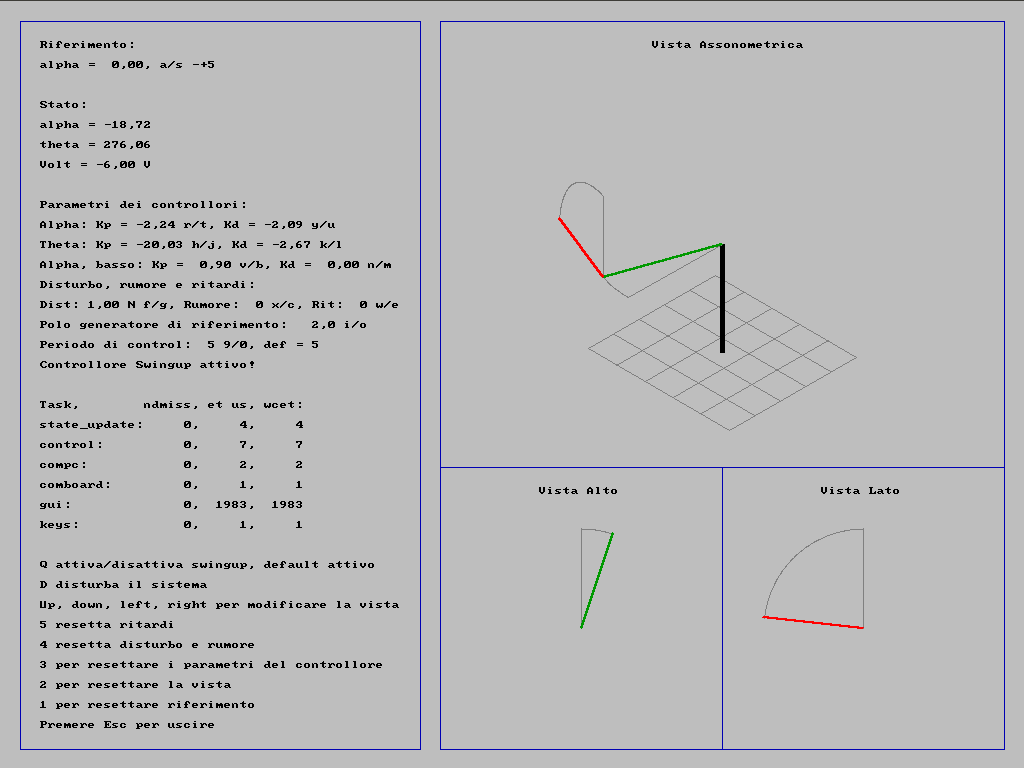
\includegraphics[height=.4\textheight]{interfaccia_in_esecuzione.png}
	\caption{Interfaccia durante l'esecuzione}
	\label{fig:interfaccia_in_esecuzione}
\end{figure}

L'interfaccia \`e divisa in due zone principali: quella di comunicazione con l'utente e le tre viste del pendolo.
Per quanto riguarda la zona di comunicazione questa \`e popolata dalle variabili di interesse e di come modificarle. Si \`e quindi riportato a schermo:
\begin{itemize}
	\item il riferimento su $\alpha$
	
	\item  il vettore di stato $\left[ \alpha \ \theta \ volt\right]^T$
	
	\item i parametri di controllo
	
	\item disturbo, rumore e ritardi
	
	\item polo della funzione di trasferimento che genera il riferimento su $\alpha$
	
	\item periodo del task di \textbf{controllo}
	
	\item per ciascun task il numero di deadline miss, il tempo di esecuzione in $\si{\micro \second}$ e il worst-case execution time in $\si{\micro \second}$
	
	\item varie istruzioni su come resettare e come uscire dal programma
	
\end{itemize}

Per quanto riguarda le viste, queste sono tre. La vista dall'alto evidenzia il primo link e quindi \`e possibile vedere $\alpha$ e il suo riferimento mentre in quella da lato $\theta$ e relativo riferimento.

\begin{figure}
	\centering
	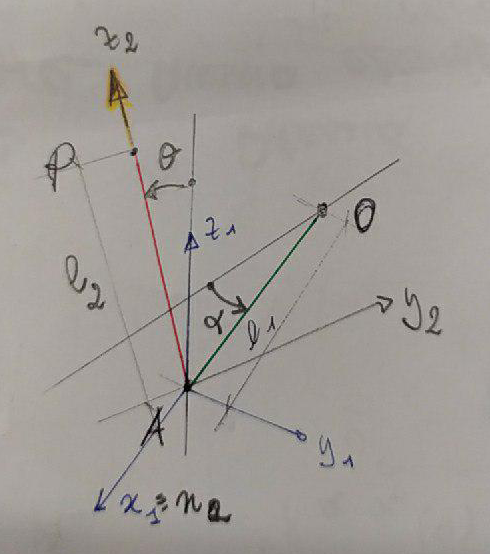
\includegraphics[height=.4\textheight]{pendolo_schema_TEMPORANEO.png}
	% MANCA DA DISEGNARCI IL SISTEMA DI RIFERIMENTO FISSO 0
	\caption{Schema del Pendolo}
	\label{fig:pendolo_schema}
\end{figure}

Per costruire la vista assonometrica \`e stato utile strutturare il problema in coordinate omogenee e introdurre dei sistemi di riferimento. Con riferimento alla figura~\ref{fig:pendolo_schema}, intendendo con $R_i(\varphi)$ la generica rotazione intorno all'asse $i$ di un angolo $\varphi$ e con $T_{ij}$ la trasformazione in coordinate omogenee dal sistema di riferimento $i$ a quello $j$ tale che per un generico vettore $p$ valga: $p_i = T_{ij} p_j$; si pu\`o elaborare i cambi di coordinate necessari. 

\begin{equation}
T_{01}(\alpha) = \quad T_{12}(\vartheta) =
\label{eq:cambio_coordinate}
\end{equation}

aaa


\begin{align}
	\mathrm{OA}& = T_{01}(\alpha) \begin{bmatrix} 0& 0 & 0& 1 \end{bmatrix}^\mathsf{T}\label{eq:from_punti_in_coord_0} \\
	\mathrm{AP}& = T_{12}(\vartheta) \begin{bmatrix}Id & 000l_2\\ 0 &1\end{bmatrix} \\
	\mathrm{OP}& = \mathrm{OA}+\mathrm{AP}
\label{eq:to_punti_in_coord_0}
\end{align}



\begin{equation}
R_{s0} = R_z (\rho)  R_y (-\lambda)  \begin{bmatrix}
0 & 0 & -1\\
1 & 0 & 0\\
0 & -1 & 0
\end{bmatrix}
\label{eq:proiezione}
\end{equation}




$\lambda$ angolo latitudine , $\rho $ angolo longitudine, da~\ref{eq:from_punti_in_coord_0}  a~\ref{eq:to_punti_in_coord_0}

% da decidere quanto entrare nel dettaglio

\section{Implementazione/code overview}
Da scrivere
\subsection{Task}
Da scrivere

\section{Conclusioni (?)}
Da Scrivere

	
\end{document}